

We will see several definitions for the  curvature of a curve or surface at a point.
Some definitions lend themselves to computations and others provide
more geometric intuition.
What  do we require of a definition of curvature?
A straight line should have zero curvature and
 large circles should have less curvature than smaller circles.
Differentiaing between
curving to the left and curving to the right will also be useful.

For any point on a one dimensional curve
we can approximate the curve with a circle.
The best approximating circle is the  \EMPH{osculating circle}.
A natural definition of the \EMPH{curvature} is the inverse of the radius of the osculating
 circle $k=\frac{1}{r}$.
See \figref{osculating-circle} for an example.
In the plane, we determine the sign of the curvature by which side of the curve the osculating circle is on.
 This osculating-circle idea can be extend
to  surfaces in $\R^3$, by considering the \EMPH{osculating sphere},
But notice that at saddle points on a surface it is not clear which sphere
best approximates the surface.
The above definition provides great intuition for the curvature of curves
and surfaces.
Computing this value depends on how a curve or surface is represented. 

\begin{figure}[htb]
	\centering
	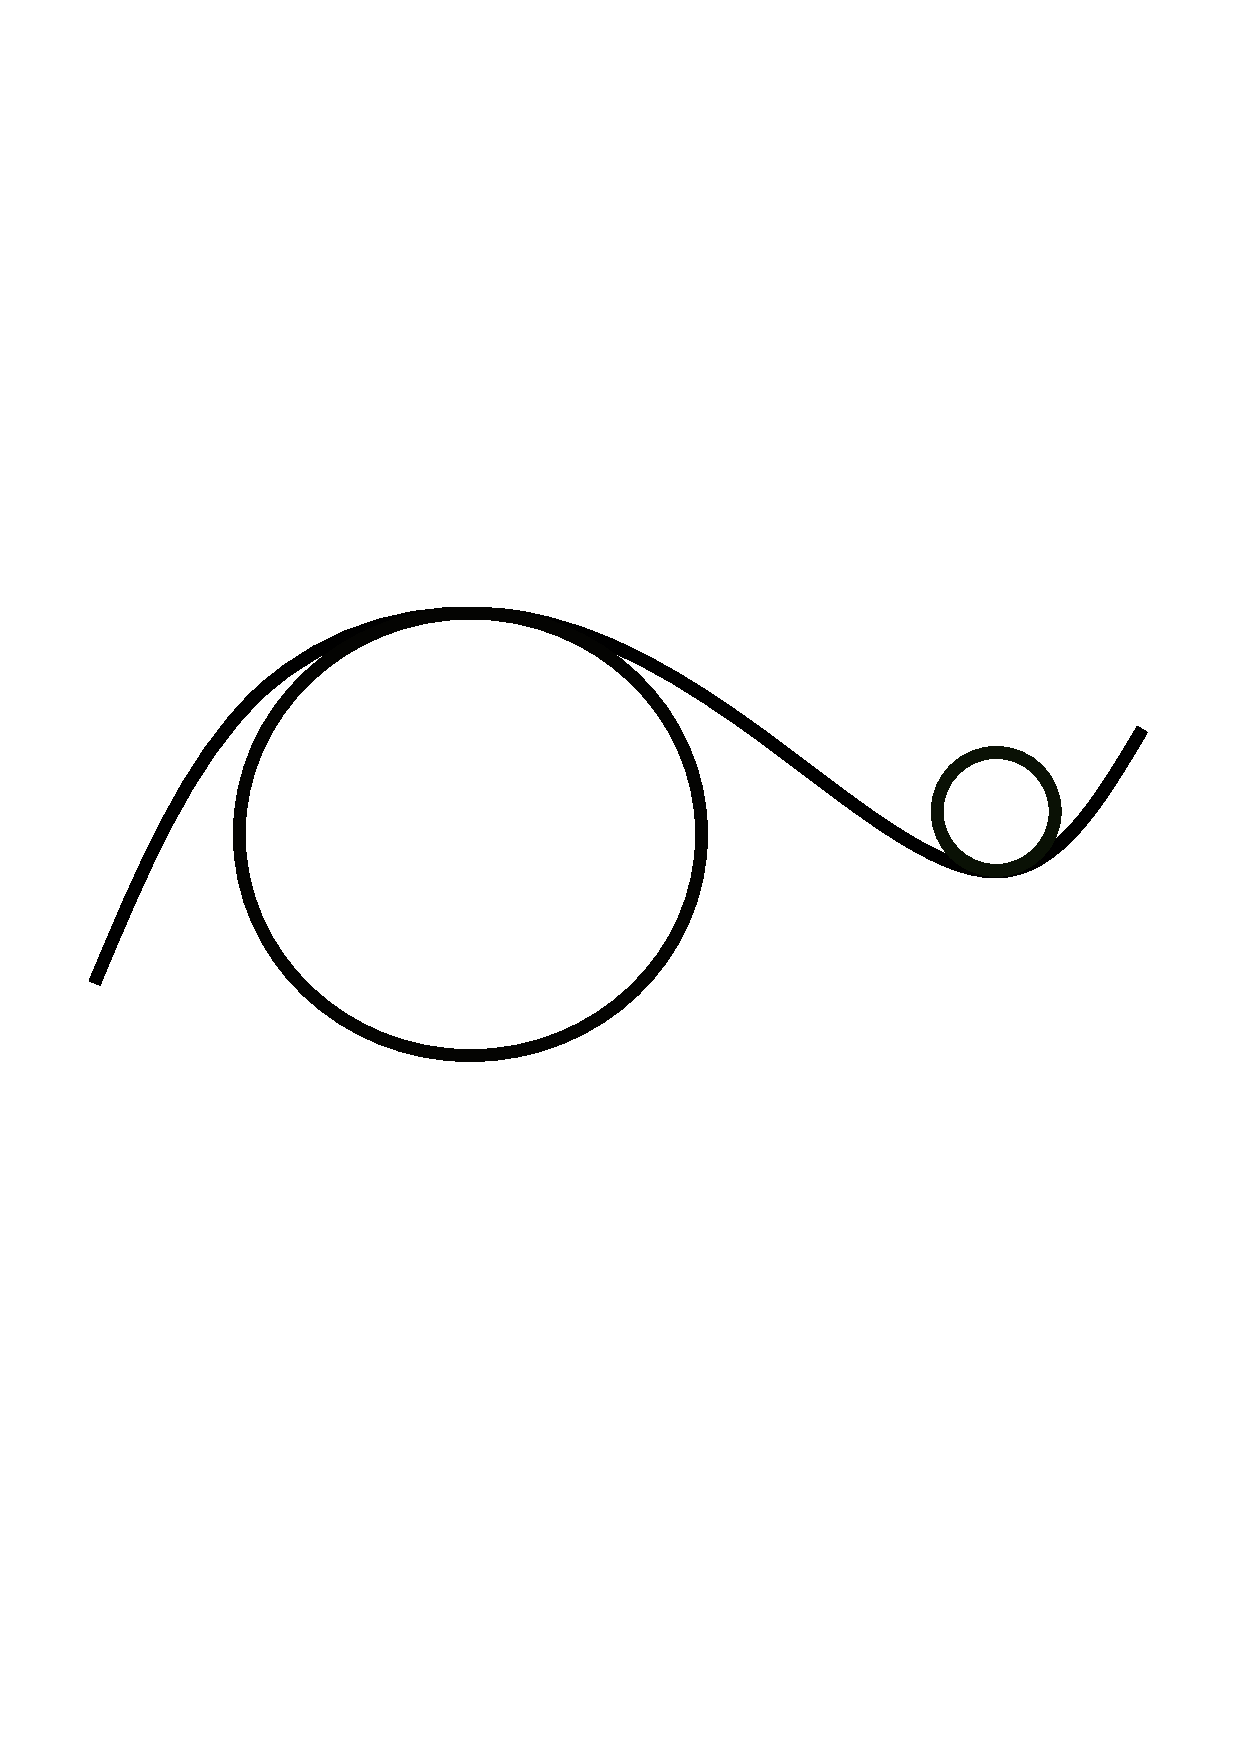
\includegraphics[width=.3\textwidth]{curvature/osculating}
	\caption{A curve with two osculating circles. The curvature at these points
	have opposite sign.}
	\label{fig:osculating-circle}
\end{figure}

A curve in $\RR^3$ is often presented as a function
$\gamma(t)=(x(t),y(t),z(t))$. We say that a curve is \EMPH{smooth} on an open interval $I$
if $\gamma'$ it is continuous and $\gamma'(t)\neq (0,0,0)$ on $I$. 
If $\gamma$ is smooth it has a well-defined unit tangent vector $T(t)=\frac{\gamma'(t)}{|\gamma'(t)|}.$
A second way to define the  \EMPH{curvature} at a point is as the magnitude of the rate of change of the 
unit tangent vector

\begin{equation} \label{eqn:kappa}
\kappa= | T'(t)|.
\end{equation}
where $t$ is arc length.

For example, take a circle of radius $r$, parameterized by 
$$C(t)=\left(r\cos(t),r\sin(t),0\right).$$
We have 
$$\frac{dC}{dt}=C'(t)=\left(-r\sin(t),r\cos(t),0\right)$$ and $|C'(t)|=r.$
Then $T(t)=\left(-\sin(t),\cos(t),0\right)$ and
$T'(t)=\left(-\cos(t),-\sin(t),0\right)$.
So, $\kappa(t)=\frac{1}{r}$ and, in this case, our definition of curvature agrees with the
osculating circle intuition given above. 
\eqnref{kappa} can be rewritten in the following more computational friendly form 
\begin{equation} \label{eqn:kappa1}
\kappa(t)=\frac{|\gamma'(t)\times \gamma''(t)|}{|\gamma'(t)|^3}.
\end{equation}

Since we traverse $\gamma$
at unit speed, $\gamma'(t)^2=1,$ and by the chain rule, $\gamma'\cdot \gamma''=0,$
so  the second derivative is orthogonal to $\gamma'$. Thus, the
vector $\gamma''=N$ is normal to the $\gamma$. 
By taking the cross product of $N$ and $T$ we obtain a vector $B$ called
the binormal vector.
The vectors $T,N$ and $B$ form the \EMPH{Fernet frame} of $\gamma$ a $p.$

\subsubsection{Surfaces}


One dimensional curves are represented by differentiable 
parameterized functions $\gamma:I\subset \RR\to \RR^3$,
we would now like to parameterize a surface.
Similarly, a \EMPH{parameterized surface} $S$ is a differentiable map $\phi:U\subset \RR^2 \to \RR^3$,
 where every point in $S$ is contained in the domain of at least one map.
These maps are called \EMPH{charts}.
% The set $\phi(U)\subset \RR^3$ is called the \EMPH{trace} of $\phi$.
If the differential $d\phi_q:\RR^2\to \RR^3$ is one-to-one for all $q\in U$ then
we say $\phi$ is \EMPH{regular}. In other words, let $(u,v)$ be coordinates of $U\subset \RR^2,$
a surface is regular if $\frac{\partial\phi}{\partial u}$
and $\frac{\partial\phi}{\partial v}$ are linearly independent for all $p\in U$.


A \EMPH{tangent vector} to $S$ at $p$ is a map $\xi:(-\epsilon,\epsilon)\to S$ with $\xi(0)=p$.
The set of all tangent vectors is the \EMPH{tangent plane} and it corresponds to the image
of the differential map $d\phi_q(\RR^2)\subset \RR^3$ (prop. 1 \cite{doc76}).
By choosing two linearly independent paths through $p\in S$ we obtain a basis 
for the tangent
plane and define a normal vector $N$ at $p$.
Every plane containing the normal vector will intersect the surface.
The intersection of the surface and each normal plane is a curve in $\RR^3$
gives a one dimensional curve called the \EMPH{normal section}. 
Let $\kappa_1$ denote the maximum curvature of all normal sections 
and let $\kappa_2$ denote the minimum. 
The \EMPH{Gaussian curvature} of a point on a surface is
$K=\kappa_1\kappa_2.$
One can check that the Gaussian curvature of the plane is zero and
that larger circles have less curvature than smaller ones.

Once we choose a chart we define a clockwise orientation to be positive.
 If the clockwise
orientation can be consistently extended to the entire surface, we say
the surface is \EMPH{orientable}.
In one dimension, the curvature is the rate of change of the tangent vector.
For an orientable surface $S$, we consider the rate of change of the normal vector.
This vector is given by the map  $N:S\to \Sp^2$ that sends each
normal in $S$ to the corresponding point on $\Sp^2$ is
the \EMPH{Gauss map}.
The determinant of the derivative of the Gauss map, $dN(p)$ quantifies the rate of change of
the normal vector ($dN$ is often called the \emph{Weingarten map} \cite{Crane:2013}).
Thus, $dN_p:T_p(S)\to T_{N(p)}(\Sp^2)$, but since $T_p(S)$ and $T_{N(p)}(\Sp^2)$
are parallel we can define $dN_p$ to be a linear map on $T_p(S)$.
The determinant of $dN(p)$ is equal to \EMPH{Gaussian curvature}.



Regular surfaces are often presented as a function as $r(u,v)=(u,v,r(u,v))$
with $u,v\in(-1,1)$.
The curvature of a surface can be thought of as a the inverse of
the radius of the osculating sphere. For example, the two sphere can be expressed
as quadratic equations $\Sp^2=(u,v,\pm\sqrt{1-u^2-v^2})$.  In general
 \EMPH{quadratic form} to be polynomial of degree two, of the form $p(u,v)=c_1u^2+c_2uv+c_3v^2$ 
where $c_i\in R$.
We define a quadratic form using $r(u,v)$ in order to compute the Gaussian curvature.


Given a `small' parallelogram $G$ on $S$ with corners $r(u,v),r(u+\epsilon u, v), r(u,v+\epsilon v)$ 
and $r(u+\epsilon u, v+\epsilon v)$ we consider the area of this parallelogram.
The unit normal vector at $p$ is given by $$n(p)=\frac{r_u\times r_v}{|r_u\times r_v|}.$$
Given a parameterized curve $u=u(t), v=v(t)$ on a regular surface, let
$s$ denote the arc length, then 
$$ds=\bigg | \frac{dr}{dt}\bigg | dt = \bigg | r_u\frac{du}{dt}+r_v\frac{dv}{dt}\bigg |dt
=\sqrt{(r_u^2 du^2+2r_ur_v du dv + r_v^2dv^2)}.$$
Let $E=r_u\cdot r_u, F=r_u\cdot r_v$ and  $G=r_v\cdot r_v$.
The rate of change of the area of $G$ is 
$$dA=\sqrt{EG-F^2}dudv.$$
And $\mathrm{I}=ds^2=Edu^2+2Fdudv +Gdv^2$ is called the \EMPH{first fundamental form}.
We summerize the first fundamental form as a matrix $\mathrm{I}=\begin{bmatrix}
E & F \\
F & G 
\end{bmatrix}.$
We get a notion of length in the tangent space, an inner product on $Tp(S)$.
If $x$ and $y$ are two tangent vectors
then $\mathrm{I}(x,y)=x^T\begin{bmatrix}
E & F \\
F & G 
\end{bmatrix}y.$


In order to compute the Gaussian curvature, we
need the second derivative.
Let $L=r_{uu}\cdot n, M=r_{uv}\cdot n$ and $N=r_{vv}\cdot n$ the
\EMPH{second fundamental form} is $\mathrm{I\!I}=Ldu^2+2Mdudv+Ndv^2$,
in matrix form $\mathrm{I\!I}=\begin{bmatrix}
L & M \\
M & N 
\end{bmatrix}.$
Another inner product is given by $\mathrm{I\!I}(x,y)=x^T\begin{bmatrix}
L & M \\
M & N 
\end{bmatrix}y.$
Then the Gaussian curvature of a surface is also given by
\begin{equation}\label{eqn:curve-dets}
 	K=\frac{\det(\mathrm{I\!I})}{\det(\mathrm{I})}.
\end{equation}


\begin{example}[Stereographic Projection \cite{christian-notes}]\label{ex:stereo}
Consider the two sphere with the north pole removed $\Sp^2 \setminus (0,0,1)$,
stereographic projection is a bijection between the points on $\Sp^2 \setminus (0,0,1)$ to the $\R^2$.
Consider a line from the north pole $(0,0,1)$ that intersects $(x,y,z)\in \Sp^2$ parametrized by 
$p(t)=(1-t)(0,0,1)+t(x,y,z)$. By considering the $z$ coordinate we determine the $t$ value where this line
intersects $\R^2$, namely $t=\frac{1}{1-z}.$
This gives the desired map shown in \figref{stereo} and in equation form
$$p(x,y,z)\to \left(\frac{x}{1-z},\frac{y}{1-z}\right).$$

\begin{figure}[htb]
	\centering
	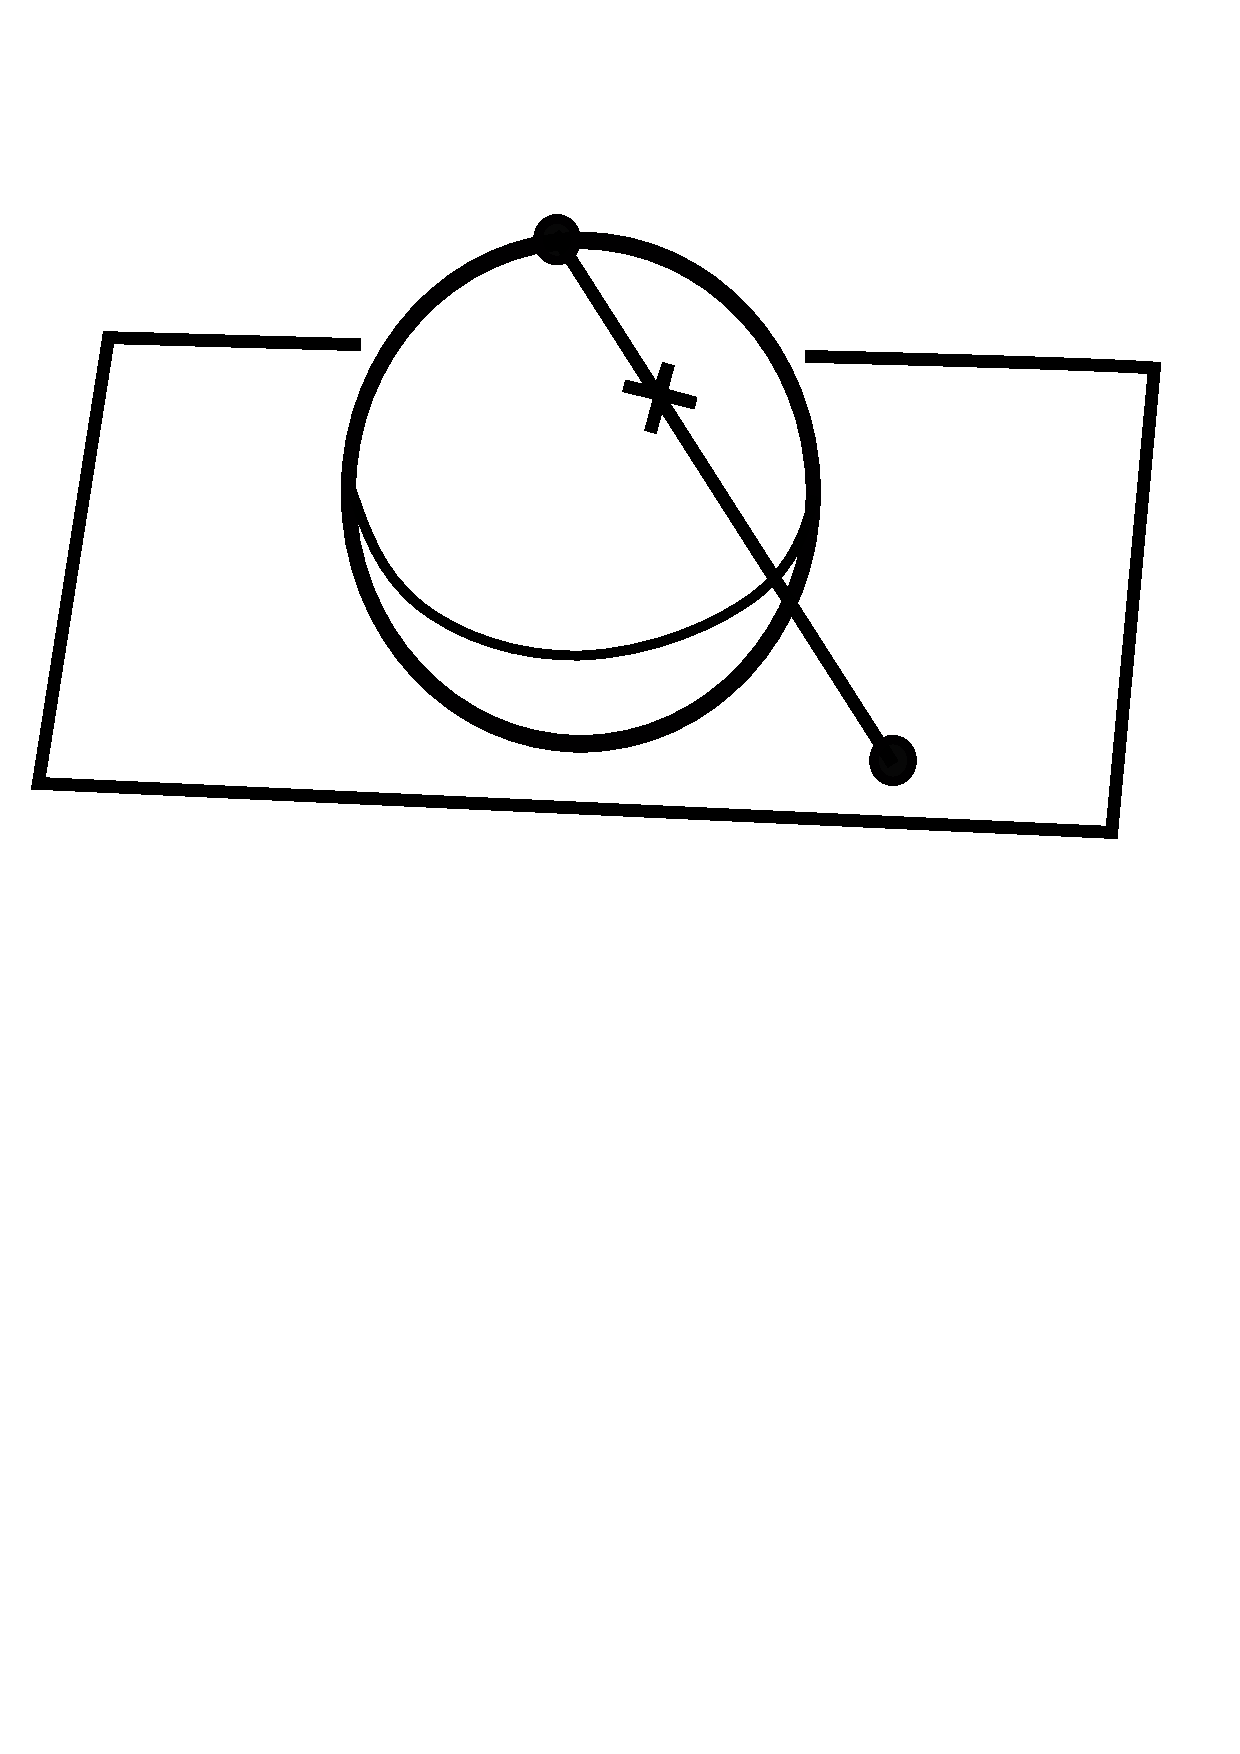
\includegraphics[width=.3\textwidth]{curvature/stereo}
	\caption{A point on the sphere is mapped to a point on the plane by stereographic projection.}
	\label{fig:stereo}
\end{figure}
	
The inverse is given by $p^{-1}:\R^2\to \R^3$

	\begin{equation}\label{eqn:stereo}
		p^{-1}(u,v)=\left(\frac{2u}{u^2+v^2+1},\frac{2v}{u^2+v^2+1},\frac{u^2+v^2-1}{u^2+v^2+1}\right).	
	\end{equation}
To compute the first fundamental form of $p^{-1}(u,v)$ we take the partial derivatives

$$p^{-1}_u=\left(\frac{2v^2-2u^2+2}{(u^2+v^2+1)^2},\frac{-4uv}{(u^2+v^2+1)^2},\frac{4v}{(u^2+v^2+1)^2}\right)$$
and 
$$p^{-1}_v=\left(\frac{-4uv}{(u^2+v^2+1)^2},\frac{2v^2-2u^2+2}{(u^2+v^2+1)^2},\frac{4v}{(u^2+v^2+1)^2}\right).$$
Then, after some algebra,
$$E=p^{-1}_u\cdot p^{-1}_u=\frac{4}{(u^2+v^2+1)^2}$$
$$F=p^{-1}_v\cdot p^{-1}_v=\frac{4}{(u^2+v^2+1)^2}$$
and
$$M=p^{-1}_u\cdot p^{-1}_v=0.$$

We can use the first fundamental form to compute
the  arc length of circles on the sphere parallel to the $xy$ plane with fixed height $z=c$ for $-1<c<1$.
This length can be computed using
the pythagorean theorem. We will see that using stereographic projection
and the first fundamental form we get the same answer.
First, use the map $p$ to map such a circle to the plane.
Using \eqnref{stereo}, our circle on the sphere maps 
to a circle in the plane because
	$$p^{-1}(u,v)=\frac{u^2+v^2-1}{u^2+v^2+1}=c$$
and we can compute the radius in terms of $c$
\begin{equation}\label{eqn:radius}
	u^2+v^2=\frac{1+c}{1-c}=k^2.
\end{equation}
	
In the plane, $u^2+v^2=k^2$ can be parameterized
as $$\gamma(t)=(k\cos(t),k\sin(t))$$ with $0\leq t\leq 2\pi.$
So our curve becomes $p^{-1}\circ \gamma(t)$ on the sphere.
Computing the partial derivatives of $\gamma(t)$ gives
$$\gamma_u'=-k\sin(t)\hspace{1.3cm}  \gamma_v'=k\cos(t).$$
Now we use the first fundamental form

$$\int_{p^{-1}}\gamma ds=\int_{0}^{2\pi} ||(p^{-1}\circ \gamma)'(t)dt=\int_0^{2\pi}\sqrt{E(\gamma_u'(t))^2+2M\gamma_u'\gamma_v'+
F(\gamma_v'(t))^2}dt.$$
Substituting and simplifying using $E=F$ we obtain
$$\int_0^{2\pi}\frac{2k}{k^2+1}dt=\frac{4\pi k}{k^2+1}.$$
Simplifying further using \eqnref{radius}  our arc length is
$$2\pi\sqrt{1-c^2}.$$

\end{example}

\todo{Do we need this? Let $S_1$ and $S_2$ be two surfaces with $\sigma:V\subset S_1\to S_2$ a differentiable map.
At $p\in S_1$ the map $d\sigma_p:T_p(S_1)\to T_{\sigma(p)}(S_2)$ is called the
\EMPH{differential} of $\sigma$ at $p$.}


Given two curves on the sphere that intersect linearly independently at a point $p$, 
stereographic projection preserves the angle between the curves.
Maps that preserve angles in this way are called \EMPH{conformal}.
We can use conformal maps to obtain a useful formula for curvature.
We follow the derivation given in $\S$ 13.1.3 of \cite{dubrovin_modern_1984}.

Let $S$ be a surface in $\R^3$ parameterized by
$$x=x(p,q), \hspace{1cm}  y=y(p,q)  \hspace{1cm} z=z(p,q).$$
Then, using the  first fundamental form, we have a metric on the surface in $\R^3$
$$d\ell^2=E(du)^2+2Fdudv + G(dv)^2$$
with $g=EG-F^2>0.$ 
We omit the proof of the following, there exists local coordinates $u,v$ for the surface with a metric of the form
$$d\ell^2=f(u,v)(du^2+dv^2).$$ 

We can then compute the curvature using this metric


\begin{theorem}[Gaussian Curvature]\label{thm:log-curve}
	Let $u,v$ be conformal coordinates of a surface $S\subset \R^3$ with
	induced metric 
	$$d\ell^2=g(u,v)(du^2+dv^2),$$
	then Gaussian curvature,  is 
		\begin{equation}\label{eqn:log-curve}
			K=\frac{-1}{2g(u,v)}\Delta(\log g(u,v))
		\end{equation}
		where $\Delta=\frac{\partial^2}{\partial u^2}+\frac{\partial^2}{\partial v^2}$
		is the Laplacian.
\end{theorem}
\begin{proof}
	Let the surface be given by local conformal coordinates $u,v$
	with $r=r(u,v)$ and $r=(x,y,z)$ in $\R^3$ coordinates.
	Our metric is given by $d\ell^2=g(u,v)(du^2+dv^2)$
	we have 
	
	\begin{equation}\label{eqn:log-curve-proof-inners}
		\langle r_u,r_u\rangle = \langle r_v,r_v\rangle=g(u,v), \hspace{1cm} \langle r_u,r_v\rangle 0.
	\end{equation}
	Differentiating with respect to $u$ and $v$ we have
	\begin{equation}\label{eqn:log-curve-proof-firsts}
		\frac{ \partial g(u,v)}{2\partial u}=\langle r_{uu}, r_u\rangle =\langle r_{uv}, r_v\rangle,
		\frac{ \partial g(u,v)}{2\partial v}=\langle r_{vv}, r_u\rangle =\langle r_{uv}, r_u\rangle
		\end{equation}
		and
		\begin{equation}\label{eqn:log-curve-proof-firsts-1}
		\langle r_{uu},r_v\rangle + \langle r_u, r_{uv}\rangle=0=\langle r_{uv},r_v\rangle + \langle r_u, r_{vv}\rangle.
		\end{equation}
	
	
	By \eqnref{log-curve-proof-inners} we can now define an orthonormal set of vectors
	\begin{equation}\label{eqn:log-curve-proof-orthog}
		e_1=\frac{r_u}{\sqrt{g(u,v}}, e_2=\frac{r_v}{\sqrt{g(u,v}}, n=[e_1,e_2].
	\end{equation}
	with $e_1$ and $e_2$ tangent to the surface.
	
	Then using the second fundamental form we have
	$$L=\langle r_{uu},n\rangle , M=\langle r_{uv},n\rangle, N=\langle r_{vv},n\rangle.$$
	Relative to $e_1, e_2$ and $n$ we have
	
	\begin{equation}\label{eqn:log-curve-proof-seconds}
		r_{uu}=\left(\frac{1}{2\sqrt{g}}\frac{\partial g}{\partial u},\frac{-1}{2\sqrt{g}}\frac{\partial g}{\partial v},L\right),\\
		r_{uv}=\left(\frac{1}{2\sqrt{g}}\frac{\partial g}{\partial v},\frac{1}{2\sqrt{g}}\frac{\partial g}{\partial u},M\right),\\
		r_{uv}=\left(\frac{-1}{2\sqrt{g}}\frac{\partial g}{\partial u},\frac{1}{2\sqrt{g}}\frac{\partial g}{\partial v},N\right).
	\end{equation}
	Then
	$$\langle r_{uu},r_{vv}\rangle -\langle r_{uv},r_{uv}\rangle=LN-M^2-\frac{1}{2g}\left[\left(\frac{\partial g}{\partial v}\right)^2+
	\left(\frac{\partial g}{\partial u}\right)^2\right]$$
	and by \eqnref{log-curve-proof-firsts-1}, we have
	$$\frac{\partial^2 g}{2\partial u^2}=\langle r_{uuv},r_{v}\rangle+\langle r_{uv},r_{uv}\rangle$$
	$$=\frac{\partial}{\partial v}\langle r_{uu},r_{v}\rangle - \langle r_{uu},r_{vv}\rangle+\langle r_{uv},r_{uv}\rangle$$
	$$=-\frac{1}{2}\frac{\partial^2 g}{\partial v^2}-(LN-M^2)+\frac{1}{2g}\left[\left(\frac{\partial g}{\partial v}\right)^2+
	\left(\frac{\partial g}{\partial u}\right)^2\right].$$
	
	Then using the definition of curvature in terms of the first and second fundamental, \eqnref{curve-dets},
	we have
	$$K=\frac{LN-M^2}{g(u,v)^2}=\frac{-1}{2g(u,v)}\Delta \ln g(u,v)$$
	as desired.
\end{proof}

\subsubsection{Geodesics Curvature}

Shortest paths play an important role in many computational problems.
In a surface, a \EMPH{geodesic} is a curve that is a shortest path
between two points in the surface. 
For example, on $\Sp^2$ great circles are geodesic.
We would like to define the curvature of a one dimensional curve as it would
 be seen from someone living on a surface.

Let $U$ be a parameterized chart on a surface $S$ with vector $n(u,v)$ normal
to the surface
and let $\gamma(t)$ be a curve in $U$, with Frenet frame $T,N,B$.
Then $V=n(\gamma(t)\times T$ is in the tangent plane of the surface since
it is perpendicular to $n$. We now have a new orthonormal basis at a point on $\gamma$
namely, $T,V,n$. 
We would like to measure how the rate of change of the tangent vector $T$ with respect to $V$.
The \EMPH{geodesic curvature} is  
\begin{equation} \label{eqn:geodesic}
	k_g=\langle \gamma''(t),V(t)\rangle
\end{equation}
For an alternative equivalent definition see \cite{doc76}.
\todo{non great circle on sphere image}



